%
% chapter.tex
%
% (c) 2020 Prof Dr Andreas Müller, Hochschule Rapperswil
%
\chapter{Permutationen
\label{buch:chapter:permutationen}}
\lhead{Permutationen}
\rhead{}
Die Berechnung der Determinante einer Matrix macht ausgedehnten
Gebrauch von der Tatsache, dass die Vertauschung von zwei Zeilen
oder Spalten das Vorzeichen des Wertes der Determinanten dreht.
In diesem Kapitel sollen die Permutationen der Zeilen abstrakt
untersucht werden.
Wir erhalten so eine abstrakte Permutationsgruppe.
Ihre Elemente lassen sich auch durch spezielle Matrizen beschreiben,
eine Darstellung dieser Gruppe, die auch unmittelbar zu einer
Formel für die Determinante einer Matrix führt.

%
% endlich.tex -- Permutationen einer endlichen Menge
%
% (c) 2020 Prof Dr Andreas Müller, Hochschule Rapperswil
%
\section{Permutationen einer endlichen Menge
\label{buch:section:permutationen-einer-endlichen-menge}}
\rhead{Permutationen}
Eine endliche Anzahl $n$ von Objekten können auf $n!$ Arten angeordnet
werden.
Da es in dieser Diskussion nicht auf die Art der Objekte ankommt,
nehmen wir als Objektmenge die Zahlen $[n] = \{ 1,\dots,n\}$
(siehe auch Definition~\ref{buch:zahlen:def:[n]}).
Die Operation, die die Objekte in eine bestimmte Reihenfolge bringt,
ist eine Abbildung $\sigma\colon[n]\to[n]$.

\begin{definition}
\label{buch:permutationen:def:permutation}
Eine {\em Permutation} ist eine umkehrbare Abbildung $[n]\to[n]$.
\index{Permutation}
Die Menge $S_n$ aller umkehrbaren Abbildungen $[n]\to[n]$
mit der Verknüpfung von Abbildungen als Operation heisst die
die {\em symmetrische Gruppe}.
\index{symmetrische Gruppe}%
Die identische Abbildung $\sigma(x)=x$ ist das {\em neutrale
Element} der Gruppe $S_n$ und wir auch mit $e$ bezeichnet.
\index{neutrales Element}%
\end{definition}

\subsection{Permutationen als $2\times n$-Matrizen}
Eine Permutation kann als $2\times n$-Matrix geschrieben werden:
\begin{center}
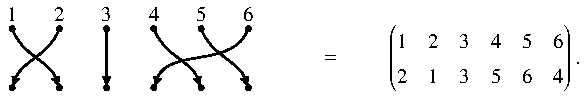
\includegraphics{chapters/50-permutationen/images/permutation.pdf}
\end{center}
Das neutrale Element hat die Matrix
\[
e = \begin{pmatrix}
1&2&3&4&5&6\\
1&2&3&4&5&6
\end{pmatrix}
\]
aus zwei identischen Zeilen.

Die Verknüpfung zweier solcher Permutationen kann leicht graphisch
dargestellt werden: dazu werden die beiden Permutationen
untereinander geschrieben und Spalten der zweiten Permutation
in der Reihenfolge der Zahlen in der zweiten Zeile der ersten
Permutation angeordnet.
Die zusammengesetzte Permutation kann dann in der zweiten Zeile
der zweiten Permutation abgelesen werden:
\begin{center}
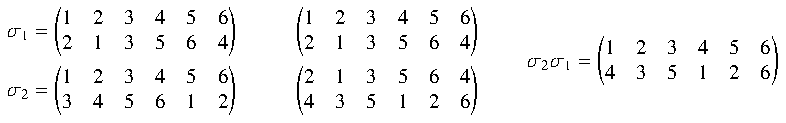
\includegraphics{chapters/50-permutationen/images/komposition.pdf}
\end{center}
Die Inverse einer Permutation kann erhalten werden, indem die beiden
Zeilen vertauscht werden und dann die Spalten wieder so angeordnet werden,
dass die Zahlen in der ersten Zeile ansteigend sind:
\[
\sigma = \begin{pmatrix}
1&2&3&4&5&6\\
2&1&3&5&6&4
\end{pmatrix}
\qquad\Rightarrow\qquad
\sigma^{-1}
=
\begin{pmatrix}
2&1&3&5&6&4\\
1&2&3&4&5&6
\end{pmatrix}
=
\begin{pmatrix}
1&2&3&4&5&6\\
2&1&3&6&4&5
\end{pmatrix}.
\]

\subsection{Zyklenzerlegung
\label{buch:subsection:zyklenzerlegung}}
Eine Permutation $\sigma\in S_n$ kann auch mit der sogenanten Zyklenzerlegung
\index{Zyklenzerlegung}%
analysiert werden.

\begin{definition}
Ein Zyklus $Z$ ist eine unter $\sigma$ invariante Teilmenge von $[n]$
minimaler Grösse.
\index{Zyklus}%
\index{invariante Teilmenge}%
\index{minimale Grösse}%
Die Zyklenzerlegung ist eine Zerlegung von $[n]$ in Zyklen
\[
[n]
=
\bigcup_{i=1}^k Z_i,
\]
wobei jede Menge $Z_i$ ein Zyklus ist.
\end{definition}

Zum Beispiel:
\begin{center}
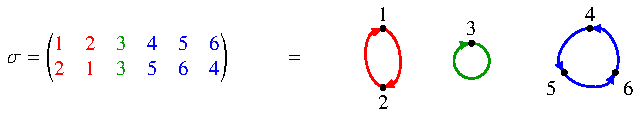
\includegraphics{chapters/50-permutationen/images/zyklenzerlegung.pdf}
\end{center}
Der folgende Satz stellt einen Algorithmus bereit, mit dem die
Zyklenzerlegung einer Permutation gefunden werden kann.

\begin{satz}
Sei $\sigma\in S_n$ eine Permutation. Der folgende Algorithmus findet
die Zyklenzerlegung von $\sigma$:
\begin{enumerate}
\item
$i=1$
\item
Wähle das erste noch nicht verwendete Element
\[
s_i=\min\biggl( [n] \setminus \bigcup_{j< i} Z_j\biggr)
\]
\item
Bestimme alle Elemente, die aus $s_i$ durch Anwendung von $\sigma$
entstehen:
\[
Z_i
=
\{ s_i, \sigma(s_i), \sigma(\sigma(s_i)), \dots \}
=
\{\sigma^k(s_i)\;|\; k\ge 0\}.
\]
\item
Falls $\bigcup_{j\le i} Z_j\ne [n]$, erhöhe $i$ um $1$ und fahre 
weiter bei 2.
\end{enumerate}
\end{satz}

Mit Hilfe der Zyklenzerlegung von $\sigma$ lassen sich auch
gewisse Eigenschaften von $\sigma$ ableiten.
Sei also $[n] = Z_1\cup\dots\cup Z_k$ die Zyklenzerlegung von $\sigma$.
Für jedes Element $x\in Z_i$ gilt $\sigma^{|Z_i|}(x) = x$.
Die kleinste Zahl $m$, für die $\sigma^m=e$ ist, das kleinste
gemeinsame Vielfache der Zyklenlängen:
\[
m = \operatorname{kgV} (|Z_1|,|Z_2|,\dots,|Z_k|).
\]
\index{kgV}
\index{kleinstes gemeinsames Vielfaches}

\subsection{Konjugierte Elemente in $S_n$}
Zwei Elemente $g_1,g_2\in G$ einer Gruppe heissen {\em konjugiert}, wenn
\index{konjugiert}
es ein Element $c\in G$ gibt derart, dass $cg_1c^{-1}=g_2$.
Bei Matrizen bedeutet dies, dass die beiden Matrizen durch
Basiswechsel auseinander hervorgehen.
Dasselbe lässt sich auch im Kontext der symmetrischen Gruppe sagen.

Seien $\sigma_1$ und $\sigma_2$ zwei konjugierte Permutationen in $S_n$.
Es gibt also eine Permutation $\gamma\in S_n$ derart, dass
$\sigma_1=\gamma\sigma_2\gamma^{-1}$ oder $\gamma^{-1}\sigma_1\gamma=\sigma_2$.
Dann gilt auch für die Potenzen
\begin{equation}
\sigma_1^k
=
(\gamma\sigma_2\gamma^{-1})^k
=
\gamma\sigma_2\underbrace{\gamma^{-1}
\gamma}_{\displaystyle=e}\sigma_2\underbrace{\gamma^{-1}
\gamma}_{\displaystyle=e}\sigma_2\underbrace{\gamma^{-1}\gamma}_{\displaystyle=e}
\cdots
\underbrace{\gamma^{-1}
\gamma}_{\displaystyle=e}\sigma_2\gamma^{-1}
=
\gamma\sigma_2^k\gamma^{-1}.
\label{buch:permutationen:eqn:konjpot}
\end{equation}
Ist $Z_i$ ein Zyklus von $\sigma_2$ und $x\in Z_i$, dann ist
$Z_i = \{ x,\sigma_2(x),\sigma_2^2(x),\dots\}$.
Die Menge $\gamma(Z_i)$ besteht dann aus dem Elementen
$\gamma(Z_i)=\{\gamma(x),\gamma(\sigma_2(x)),\gamma(\sigma_2^2(x)),\dots\}$.
Aus der Formel~\eqref{buch:permutationen:eqn:konjpot} folgt
$\sigma_1^k\gamma = \gamma\sigma_2^k$, also
\[
\gamma(Z_i)
=
\{\gamma(x),\sigma_1(\gamma(x)),\sigma_1^2(\gamma(x)),\dots\}.
\]
Somit ist $\gamma(Z_i)$ ein Zyklus von $\sigma_1$.
Die Permutation $\gamma$ bildet also Zyklen von $\sigma_2$ auf Zyklen
von $\sigma_1$ ab.
Es folgt daher der folgende Satz:

\begin{satz}
Seien $\sigma_1,\sigma_2\in S_n$ konjugiert $\sigma_1=\gamma\sigma_2\gamma^{-1}$
mit $\gamma\in S_n$.
Wenn $Z_1,\dots,Z_k$ die Zyklen von $\sigma_2$ sind, dann sind 
$\gamma(Z_1),\dots,\gamma(Z_k)$ die Zyklen von $\sigma_1$.
\end{satz}

Die Zyklenzerlegung kann mit der Jordan-Normalform
\index{Jordan-Normalform}%
(Abschnitt~\ref{buch:subsection:jordan-normalform})
einer Matrix verglichen werden.
Durch einen Basiswechsel, welcher durch eine ``Konjugation''
\index{Basiswechsel}%
von Matrizen ausgedrückt wir, kann die Matrix in eine besonders 
übersichtliche Form gebracht werden.
Wenn $\sigma$ die Zyklenzerlegung $Z_1,\dots,Z_k$ hat mit Zyklenlängen
$l_i=|Z_i|$, dann kann man die Menge $[n]$ wie folgt in Teilmengen
\begin{align*}
X_1 &= \{1,\dots, l_1\},
\\
X_2 &= \{l_1+1,\dots,l_1+l_2\},
\\
X_i &= \{l_1+\dots+l_{i-1}+1,\dots, l_1+\dots+l_i\}
\\
X_k &= \{l_1+\dots+l_{k-1}+1,\dots n\}
\end{align*}
zerlegen.
Sei $\sigma_2$ die Permutation, die in jeder der Mengen $X_i$ durch
zyklische Vertauschung der Elemente wirkt.
Indem man die Elemente von $Z_i$ in der Reihenfolge, in der sie durch
$\sigma_1$ erreicht werden, auf die Elemente $X_i$ abbildet, findet
man eine Permutation, die Zyklen von $\sigma_1$ in Zyklen von $\sigma_2$
überführt.

\begin{satz}
Wenn zwei Elemente $\sigma_1,\sigma_2\in S_n$ Zyklenzerlegungen mit den
gleichen Zyklenlängen haben, dann sind sie konjugiert.
\end{satz}

Ein Element $\sigma\in S_n$ ist also bis auf eine Permutation
vollständig durch die Länge der Zyklen von $\sigma$ charakterisiert.



%
% transpositionen.tex -- Permutationen aus Transpositionen erzeugen
%
% (c) 2020 Prof Dr Andreas Müller, Hochschule Rapperswil
%
\section{Permutationen und Transpositionen
\label{buch:section:permutationen-und-transpositionen}}
\rhead{Transpositionen}
Im vorangegangenen Abschnitt haben wir Permutationen durch die
Zyklenzerlegung charakterisiert.
Es zeigt sich aber, dass sich eine Permutation in noch elementarere
Bausteine zerlegen lässt, die Transpositionen.

\begin{definition}
Einen Transposition $\tau\in S_n$ ist ein Permutation, die genau
zwei Elemente vertauscht.
Die Transposition $\tau_{ij}$ ist definiert durch
\[
\tau_{ij}(x)
=
\begin{cases}
i&\qquad x=j\\
j&\qquad x=i\\
x&\qquad\text{sonst.}
\end{cases}
\]
\end{definition}

Eine Transposition hat genau einen Zyklus der Länge $2$, alle anderen
Zyklen haben die Länge $1$.

\subsection{Zyklus und Permutationen aus Transpositionen}
Sei $\sigma$ die zyklische Vertauschung der Elemente $1,\dots,k\in [n]$,
also die Permutation, die $1\to2\to3\to\dots\to k-2\to k-1\to k\to 1$
abbildet.
Dieser Zyklus lässt sich wie folgt aus Transpositionen zusammensetzen:
\begin{center}
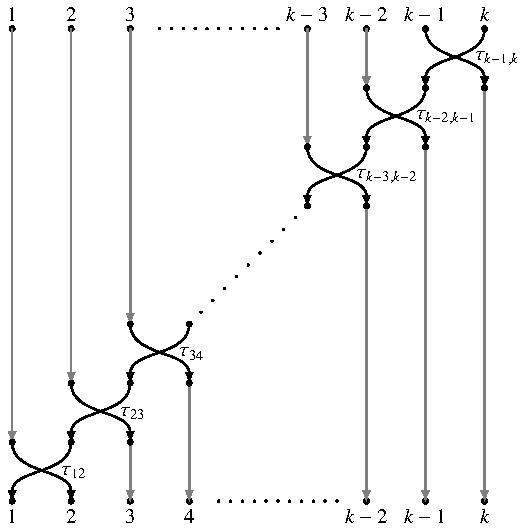
\includegraphics{chapters/50-permutationen/images/transpositionen.pdf}
\end{center}
Es ist also
\[
\sigma 
=
\tau_{12} \tau_{23} \tau_{34} \dots \tau_{k-3,k-2} \tau_{k-2,k-1} \tau_{k-1,k}.
\]
\begin{satz}
Jede Permutation $\sigma\in S_n$ lässt sich als ein Produkt von 
Transpositionen schreiben.
Jeder Zyklus der Länge $k$ lässt sich aus $k-1$ Transpositionen
zusammensetzen.
Eine Permutation mit einer Zerlegung in Zyklen der Längen $l_1,\dots,l_p$
kann als Produkt von $l_1+\dots+l_p-p$ Transpositionen geschrieben werden.
\end{satz}

\subsection{Signum einer Permutation}
Die Anzahl Transpositionen, die benötigt werden, um eine Permutation
zu beschreiben, ist nicht fest. 
Wenn $\sigma$ mit $k$ Transpositionen geschrieben werden kann und
$\gamma$ mit $l$, dann hat $\gamma\sigma\gamma^{-1}$ die gleiche
Zyklenzerlegung, kann aber mit $k+2l$ Transpositionen geschrieben
werden.
Die Anzahl Transpositionen, die zur Darstellung einer Permutation
nötig ist, ändert sich aber immer nur um eine gerade Zahl.
Die Anzahl ist also keine Invariante einer Permutation, aber ob
die Anzahl gerade ist oder nicht, ist sehr wohl eine charkterisierende
Eigenschaft einer Permutation.

\begin{definition}
Das {\em Vorzeichen} oder {\em Signum} einer Permutation $\sigma$ ist
die Zahl $\operatorname{sgn}(\sigma)=(-1)^k$, wenn $\sigma$ als Produkt
von $k$ Transpositionen geschrieben werden kann.
\end{definition}

Die inverse Permutation $\sigma^{-1}$ hat das gleiche Signum wie $\sigma$.
Wenn nämlich $\sigma= \tau_1\tau_2\dots\tau_k$ geschrieben werden kann,
dann ist $\sigma^{-1}=\tau_k\dots\tau_2\tau_1$, sowohl $\sigma$ wie
$\sigma^{-1}$ können also mit der gleichen Zahl von Transpositionen
geschrieben werden, sie haben also auch das gleiche Vorzeichen.

Die Abbildung $S_n\to\{\pm\}$, die einer Permutation das Signum zuordnet,
ist ein Homomorphismus von Gruppen,
d.~h.
\[
\operatorname{sgn}(\sigma_1\sigma_2)
=
\operatorname{sgn}(\sigma_1)
\operatorname{sgn}(\sigma_2)
\]
da ganz offensichtlich $\sigma_1\sigma_2$ mit $k_1+k_2$ Transpositionen
geschrieben kann, wenn $\sigma_i$ mit $k_i$ Transpositionen geschrieben
werden kann.

Das Signum definiert in der symmetrischen Gruppe eine Teilmenge bestehnd
aus den Permutationen mit Signum $+1$.

\begin{definition}
Die Teilmenge
\[
A_n
=
\{
\sigma\in S_n\;|\; \operatorname{sgn}(\sigma)=1
\}
\subset S_n.
\]
heisst die {\em alternierende Gruppe} der Ordnung $n$
Die Elemente von $A_n$ heissen auch die {\em geraden} Permutationen,
die
Elemente von $S_n\setminus A_n$ heissen auch die {\em ungeraden}
Permutationen.
\end{definition}

Die alternierende Gruppe $A_n$ ist tatsächlich eine Untergruppe.
Zunächst ist $\operatorname{sgn}(e)=(-1)^0=1$, also ist $e\in A_n$.
Es wurde schon gezeigt, dass mit jedem Element $\sigma\in A_n$ auch
das inverse Element $\sigma^{-1}\in A_n$ ist.
Es muss aber noch sichergestellt werden, dass das Produkt von zwei
geraden Transpositionen wieder gerade ist:
\[
\begin{aligned}
\sigma_1,\sigma_2&\in A_n
&\Rightarrow&&
\operatorname{sgn}(\sigma_1)
&=
\operatorname{sgn}(\sigma_2)
=
1
\\
&&\Rightarrow&&
\operatorname{sgn}(\sigma_1\sigma_2)
&=
\operatorname{sgn}(\sigma_1)
\operatorname{sgn}(\sigma_2)
=
1\cdot 1=1
&&\Rightarrow&
\sigma_1\sigma_2&\in A_n.
\end{aligned}
\]
Damit ist gezeigt, dass die alternierende Gruppe $A_n$ ein Untergruppe von 
$S_n$ ist.


%
% permutationsmatrizen.tex -- Permutationsmatrizen
%
% (c) 2020 Prof Dr Andreas Müller, Hochschule Rapperswil
%
\section{Permutationsmatrizen
\label{buch:section:permutationsmatrizen}}
\rhead{Permutationsmatrizen}
Die Eigenschaft, dass eine Vertauschung das Vorzeichen kehrt, ist
eine wohlebekannte Eigenschaft der Determinanten.
In diesem Abschnitt soll daher eine Darstellung von Permutationen
als Matrizen gezeigt werden und die Verbindung zwischen dem
Vorzeichen einer Permutation und der Determinanten hergestellt
werden.

\subsection{Matrizen}
Gegeben sei jetzt eine Permutation $\sigma\in S_n$. 
Aus $\sigma$ lässt sich eine lineare Abbildung $\Bbbk^n\to\Bbbk^n$
konstruieren, die die Standardbasisvektoren permutiert, also
\[
f_{\sigma}\colon
\Bbbk^n \to \Bbbk^n
:
\left\{
\begin{aligned}
e_1&\mapsto e_{\sigma(1)} \\
e_2&\mapsto e_{\sigma(2)} \\
\vdots&\\
e_n&\mapsto e_{\sigma(n)}
\end{aligned}
\right.
\]
Die Matrix $P_\sigma$ der linearen Abbildung $f_{\sigma}$ hat in Spalte $i$
genau eine $1$ in der Zeile $\sigma(i)$, also
\[
(P_\sigma)_{ij} = \delta_{j\sigma(i)}.
\]

\begin{beispiel}
Die zur Permutation
\[
\begin{pmatrix}
1&2&3&4&5&6\\
2&1&3&5&6&4
\end{pmatrix}
\]
gehörige lineare Abbildung $f_\sigma$ hat die Matrix
\[
A_\sigma
=
\begin{pmatrix}
0&1&0&0&0&0\\
1&0&0&0&0&0\\
0&0&1&0&0&0\\
0&0&0&0&0&1\\
0&0&0&1&0&0\\
0&0&0&0&1&0
\end{pmatrix}
\qedhere
\]
\end{beispiel}

\begin{definition}
Eine Permutationsmatrix ist eine Matrix $P\in M_n(\Bbbk)$ 
derart, die in jeder Zeile und Spalte genau eine $1$ enhalten,
während alle anderen Matrixelemente $0$ sind.
\end{definition}

Es ist klar, dass aus einer Permutationsmatrix auch die Permutation
der Standardbasisvektoren abgelesen werden kann.
Die Verknüpfung von Permutationen wird zur Matrixmultiplikation
von Permutationsmatrizen, die Zuordnung $\sigma\mapsto P_\sigma$
ist also ein Homomorphismus
$
S_n \to M_n(\Bbbk^n),
$
es ist $P_{\sigma_1\sigma_2}=P_{\sigma_1}P_{\sigma_2}$.

\subsection{Transpositionen}
Transpositionen sind Permutationen, die genau zwei Elemente von $[n]$
vertauschen.
Wir ermitteln jetzt die Permutationsmatrix der Transposition $\tau=\tau_{ij}$
\[
P_{\tau_{ij}}
=
\begin{pmatrix}
1&      & &      &     &      & &      & \\
 &\ddots& &      &     &      & &      & \\
 &      &1&      &     &      & &      & \\
 &      & &0     &\dots&1     & &      & \\
 &      & &\vdots&     &\vdots& &      & \\
 &      & &1     &\dots&0     & &      & \\
 &      & &      &     &      &1&      & \\
 &      & &      &     &      & &\ddots& \\
 &      & &      &     &      & &      &1
\end{pmatrix}
\qedhere
\]

Die Permutation $\sigma$ mit dem Zyklus $1\to 2\to\dots\to l-1\to l\to 1$
der Länge $l$ kann aus aufeinanderfolgenden Transpositionen zusammengesetzt
werden, die zugehörigen Permutationsmatrizen sind
\begin{align*}
P_\sigma
&=
P_{\tau_{12}}
P_{\tau_{23}}
P_{\tau_{34}}\dots
P_{\tau_{l-2,l-1}}
P_{\tau_{l-1,l}}
\\
&=
\begin{pmatrix}
0&1&0&0&\dots\\
1&0&0&0&\dots\\
0&0&1&0&\dots\\
0&0&0&1&\dots\\
\vdots&\vdots&\vdots&\vdots&\ddots
\end{pmatrix}
\begin{pmatrix}
1&0&0&0&\dots\\
0&0&1&0&\dots\\
0&1&0&0&\dots\\
0&0&0&1&\dots\\
\vdots&\vdots&\vdots&\vdots&\ddots
\end{pmatrix}
\begin{pmatrix}
1&0&0&0&\dots\\
0&1&0&0&\dots\\
0&0&0&1&\dots\\
0&0&1&0&\dots\\
\vdots&\vdots&\vdots&\vdots&\ddots
\end{pmatrix}
\dots
\\
&=
\begin{pmatrix}
0&0&1&0&\dots\\
1&0&0&0&\dots\\
0&1&0&0&\dots\\
0&0&0&1&\dots\\
\vdots&\vdots&\vdots&\vdots&\ddots
\end{pmatrix}
\begin{pmatrix}
1&0&0&0&\dots\\
0&1&0&0&\dots\\
0&0&0&1&\dots\\
0&0&1&0&\dots\\
\vdots&\vdots&\vdots&\vdots&\ddots
\end{pmatrix}
\dots
\\
&=
\begin{pmatrix}
0&0&0&1&\dots\\
1&0&0&0&\dots\\
0&1&0&0&\dots\\
0&0&1&0&\dots\\
\vdots&\vdots&\vdots&\vdots&\ddots
\end{pmatrix}
\\
&\vdots\\
&=
\begin{pmatrix}
0&0&0&0&\dots&0&1\\
1&0&0&0&\dots&0&0\\
0&1&0&0&\dots&0&0\\
0&0&1&0&\dots&0&0\\
\vdots&\vdots&\vdots&\vdots&\ddots&\vdots&\vdots\\
0&0&0&0&\dots&1&0
\end{pmatrix}
\end{align*}

\subsection{Determinante und Vorzeichen}
Die Transpositionen haben Permutationsmatrizen, die aus der Einheitsmatrix
entstehen, indem genau zwei Zeilen vertauscht werden.
Die Determinante einer solchen Permutationsmatrix ist
\[
\det P_{\tau} = - \det E = -1 = \operatorname{sgn}(\tau).
\]
Nach der Produktregel für die Determinante folgt für eine Darstellung
der Permutation $\sigma=\tau_1\dots\tau_l$ als Produkt von Transpositionen,
dass
\[
\det P_{\sigma}
=
\det P_{\tau_1} \dots \det P_{\tau_l}
=
(-1)^l
=
\operatorname{sgn}(\sigma).
\]
Das Vorzeichen einer Permutation ist also identisch mit der Determinante
der zugehörigen Permutationsmatrix.



%
% determinante.tex -- Formel für die Determinante mit Vorzeichen der
%                     Permutation
%
% (c) 2020 Prof Dr Andreas Müller, Hochschule Rapperswil
%
\section{Determinante
\label{buch:section:determinante}}
\rhead{Determinante}
Das Signum einer Permutationsmatrizen lässt sich
gemäss~\eqref{buch:permutationen:determinante}
mit der Determinanten berechnen.
Umgekehrt sollte es auch möglich sein, eine Formel
für die Determinante zu finden.
Die Basis dafür ist der
Entwicklungssatz 
\begin{equation}
\det(A)
=
\sum_{i=1}^n (-1)^{i+j} a_{i\!j} \cdot \det(A_{i\!j})
\label{buch:permutationen:entwicklungssatz}
\end{equation}
von Laplace für die Determinante.
\index{Entwicklungssatz}%
\index{Laplace, Entwicklungssatz von}%
Die Matrizen $A_{i\!j}$ sind die Minoren der Matrix $A$
(siehe auch Seite~\pageref{buch:linear:def:minor}).
In den Produkten $a_{i\!j}\cdot\det(A_{i\!j})$ enthält 
die Untermatrix $A_{i\!j}$ weder Elemente der Zeile $i$ noch der 
Zeile $j$.
Die Summanden auf der rechten Seite von
\eqref{buch:permutationen:entwicklungssatz}
sind daher Produkte der Form
\[
a_{1i_1}
a_{2i_2}
a_{3i_3}
\cdots
a_{ni_n},
\]
in denen nur Faktoren aus verschiedenen Spalten der Matrix $A$
vorkommen.
Das ist gleichbedeutend damit, dass unter den Spaltenindizes
$i_1,i_2,i_3,\dots,i_n$ keine zwei gleich sind, dass also
\[
\sigma
=
\begin{pmatrix}
1&2&3&\dots&n\\
i_1&i_2&i_3&\dots&i_n
\end{pmatrix}
\]
eine Permutation ist.

Die Determinante muss sich daher als Summe über alle Permutationen
in der Form
\begin{equation}
\det(A)
=
\sum_{\sigma\in S_n} 
c(\sigma)
\,
a_{1\sigma(1)}
a_{2\sigma(2)}
\cdots
a_{n\sigma(n)}
\label{buch:permutationen:cformel}
\end{equation}
schreiben lassen, wobei die Koeffizienten $c(\sigma)$ noch zu bestimmen
sind.
Setzt man in
\eqref{buch:permutationen:cformel}
eine Permutationsmatrix $P_\tau$ ein, dann verschwinden alle
Terme auf der rechten Seite ausser dem zur Permutation $\tau$,
also
\[
\det(P_\tau)
=
\sum_{\sigma \in S_n}
c(\sigma)
\,
(P_\tau)_{1\sigma(1)}
(P_\tau)_{2\sigma(2)}
\cdots
(P_\tau)_{n\sigma(n)}
=
c(\tau)
\,
1\cdot 1\cdots 1
=
c(\tau).
\]
Der Koeffizientn $c(\tau)$ ist also genau das Vorzeichen
der Permutation $\tau$.
Damit erhalten wir den folgenden Satz:

\begin{satz}
Die Determinante einer $n\times n$-Matrix $A$ kann berechnet werden als
\[
\det(A)
=
\sum_{\sigma\in S_n}
\operatorname{sgn}(\sigma)
a_{1\sigma(1)}
a_{2\sigma(2)}
\cdots
a_{n\sigma(n)}
=
\sum_{\tau\in S_n}
\operatorname{sgn}(\tau)
a_{\tau(1)1}
a_{\tau(2)2}
\cdots
a_{\tau(n)n}.
\]
Insbesondere folgt auch $\det(A)=\det(A^t)$.
\end{satz}



\section*{Übungsaufgaben}
\aufgabetoplevel{chapters/50-permutationen/uebungsaufgaben}
\begin{uebungsaufgaben}
\uebungsaufgabe{5001}
\end{uebungsaufgaben}

